Das $s(t)$-Diagramm (oben) beschreibt die Bewegung eines Körpers auf einer geraden Linie; es besteht aus fünf Stücken. Eine Schülerin hat dazu das $v(t)$-Diagramm (unten) skizziert. Vier Stücke ihrer Skizze sind richtig, eines ist falsch.
\begin{center}
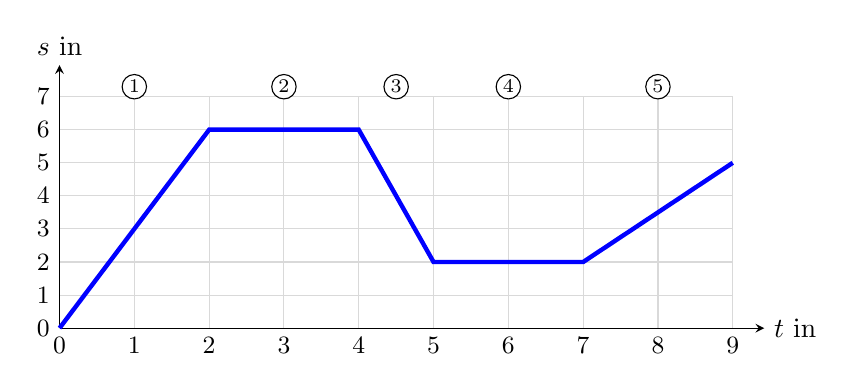
\begin{tikzpicture}[>=stealth, x=0.95cm, y=0.42cm]
 \draw[gray!30] (0,0) grid[xstep=1, ystep=1] (9,7);
 \draw[->] (0,0) -- (9.421,0) node[right] {$t$ in \si{\second}};
 \draw[->] (0,0) -- (0,7.952) node[above] {$s$ in \si{\meter}};
 \foreach \tk in {0,1,2,3,4,5,6,7,8,9} \node[below] at (\tk,0) {\small $\tk$};
 \foreach \yk in {0,1,2,3,4,5,6,7} \node[left] at (0,\yk) {\small $\yk$};
 \draw[ultra thick, blue] (0,0) -- (2,6) -- (4,6) -- (5,2) -- (7,2) -- (9,5);
 \node[circle, draw, inner sep=1pt, font=\scriptsize, fill=white] at (1,7.3) {1};
 \node[circle, draw, inner sep=1pt, font=\scriptsize, fill=white] at (3,7.3) {2};
 \node[circle, draw, inner sep=1pt, font=\scriptsize, fill=white] at (4.5,7.3) {3};
 \node[circle, draw, inner sep=1pt, font=\scriptsize, fill=white] at (6,7.3) {4};
 \node[circle, draw, inner sep=1pt, font=\scriptsize, fill=white] at (8,7.3) {5};
\end{tikzpicture}
\end{center}\begin{center}
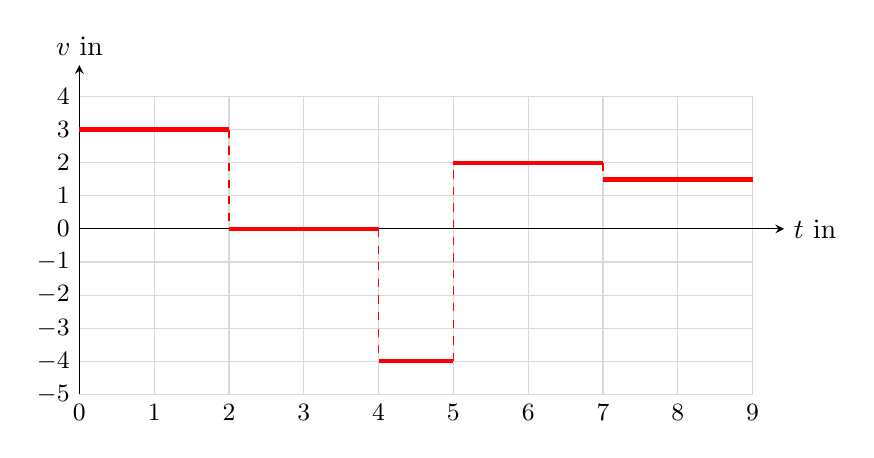
\begin{tikzpicture}[>=stealth, x=0.95cm, y=0.42cm]
 \draw[gray!30] (0,-5) grid[xstep=1, ystep=1] (9,4);
 \draw[->] (0,0) -- (9.421,0) node[right] {$t$ in \si{\second}};
 \draw[->] (0,-5) -- (0,4.952) node[above] {$v$ in \si{\meter\per\second}};
 \foreach \tk in {0,1,2,3,4,5,6,7,8,9} \node[below] at (\tk,-5) {\small $\tk$};
 \foreach \yk in {-5,-4,-3,-2,-1,0,1,2,3,4} \node[left] at (0,\yk) {\small $\yk$};

 \draw[ultra thick, red] (0,3) -- (2,3);
 \draw[ultra thick, red] (2,0) -- (4,0);
 \draw[ultra thick, red] (4,-4) -- (5,-4);
 \draw[ultra thick, red] (5,2) -- (7,2);
 \draw[ultra thick, red] (7,1.5) -- (9,1.5);
 \draw[red, dashed] (2,3) -- (2,0) (4,0) -- (4,-4) (5,-4) -- (5,2) (7,2) -- (7,1.5);
\end{tikzpicture}
\end{center}
\begin{abcliste}
\abc Welches Stück ist falsch?
\abc Welchen Fehler hat die Schülerin gemacht? Wie sieht das Stück richtig aus?
\end{abcliste}
